\setcounter{equation}{0}
\chapter{Results}
\label{chap:results}

\section{Parameters' Intial Values}

With the model defined and the code implemented, the following step is to run the simulations. It is then necessary to set values for the parameters. \\

In order to define the ranges of \tauh it is necessary to refer to observations. The literature available offers a value of LAE's Hydrogen mass that goes from $2.7\times 10^{8}$\Msun - $2.7\times 10^{9}$\Msun. These values cause a Hydrogen density of $4\times10^{-4}-4\times 10^{-3}$ $\mathrm{atoms}/\mathrm{cm}^3$, which finally translates to the ranges of optical depth: $\tau_{\rm H}=2 \times 10^{5} - 2 \times 10^{6}$. However to consider LAEs that might be more massive, I will extend this range to $\tau_{\rm H}=2 \times 10^{5} - 2 \times 10^{7}$ \\

When looking at the literature one can find typical values for both \vrot and \vout. Nonetheless, the combined effect of these two have never been studied on a LAE before. Because of this, I made a mapping of them without concerning of their physical meaning. So, all the combinations of Tab. \ref{tab:first} are executed. \\

\begin{table}[htbp]
	\centering
	\begin{tabular}{|c|c|c|}
		\hline
		\bv{\tau_{\mathrm{H}}} & \bv{v_{rot}} (\kms) & \bv{v_{out}} (\kms) \\
		\hline
		$10^5$, $10^6$, $10^7$ & 0, 100, 200 ,300 & 100, 200 ,300 \\
		\hline
	\end{tabular}
	\caption{\textbf{Combinations of parameters' values:} Rough estimation to see the effect of each parameter.}
	\label{tab:first}
\end{table}

The final results are shown in the Appendix \ref{first_plots} in Figs. \ref{fig:1_tau10E5_phi83-90}, \ref{fig:1_tau10E6_phi83-90} and \ref{fig:1_tau10E7_phi83-90}. In these three sets of figures it is noted that most of the lines are a single peaks. However, the effect of rotation should create two. Only in few squares the 2 peaks are visible but they are almost insignificant in comparison and there has to be low \vrot and \vout to obtain them. This means that the outflows effect so much larger than the other one, and in order to compare the influence of both is necessary to lower \vout. This behavior extends for all the viewing angle ranges.\\

\section{Narrowing Parameters' Values}

Knowing the typical velocity values for a LAE and that \vout has to be much lower than \vrot, the values of the parameters are narrowed. All of them are registered in Tab. \ref{tab:second}. Their combinations are executed. \\

\begin{table}[htbp]
	\centering
	\begin{tabular}{|c|c|c|}
		\hline
		\bv{\tau_{\mathrm{H}}} & \bv{v_{rot}} (\kms) & \bv{v_{out}} (\kms) \\
		\hline
		$10^5$, $10^6$, $10^7$ & 50, 100 & 5, 10, 15, 20, 25, 50, 75 \\
		\hline
	\end{tabular}
	\caption{\textbf{Combinations of parameters' values:} The velocities are now consistent with the LAE's mass and typical properties}
	\label{tab:second}
\end{table}

From these new sets of spectra I notice that \vout = 50, 75 \kms still behave as the values of the previous section. The outflows velocity is too large to let another effect be visible. These spectra are also available in the Appendix \ref{first_plots} in Figs. \ref{fig:2_tau10E5_phi83-90} \ref{fig:2_tau10E6_phi83-90} \ref{fig:2_tau10E7_phi83-90}.\\

On the other side, for the remaining values of \vout significants results are obtained. They are shown in Figs. \ref{fig:3_tau10E5_phi83-90}, \ref{fig:3_tau10E7_phi83-90} and \ref{fig:3_tau10E6_phi83-90}. 

\newpage

\begin{figure}[h!]
	\begin{center}
		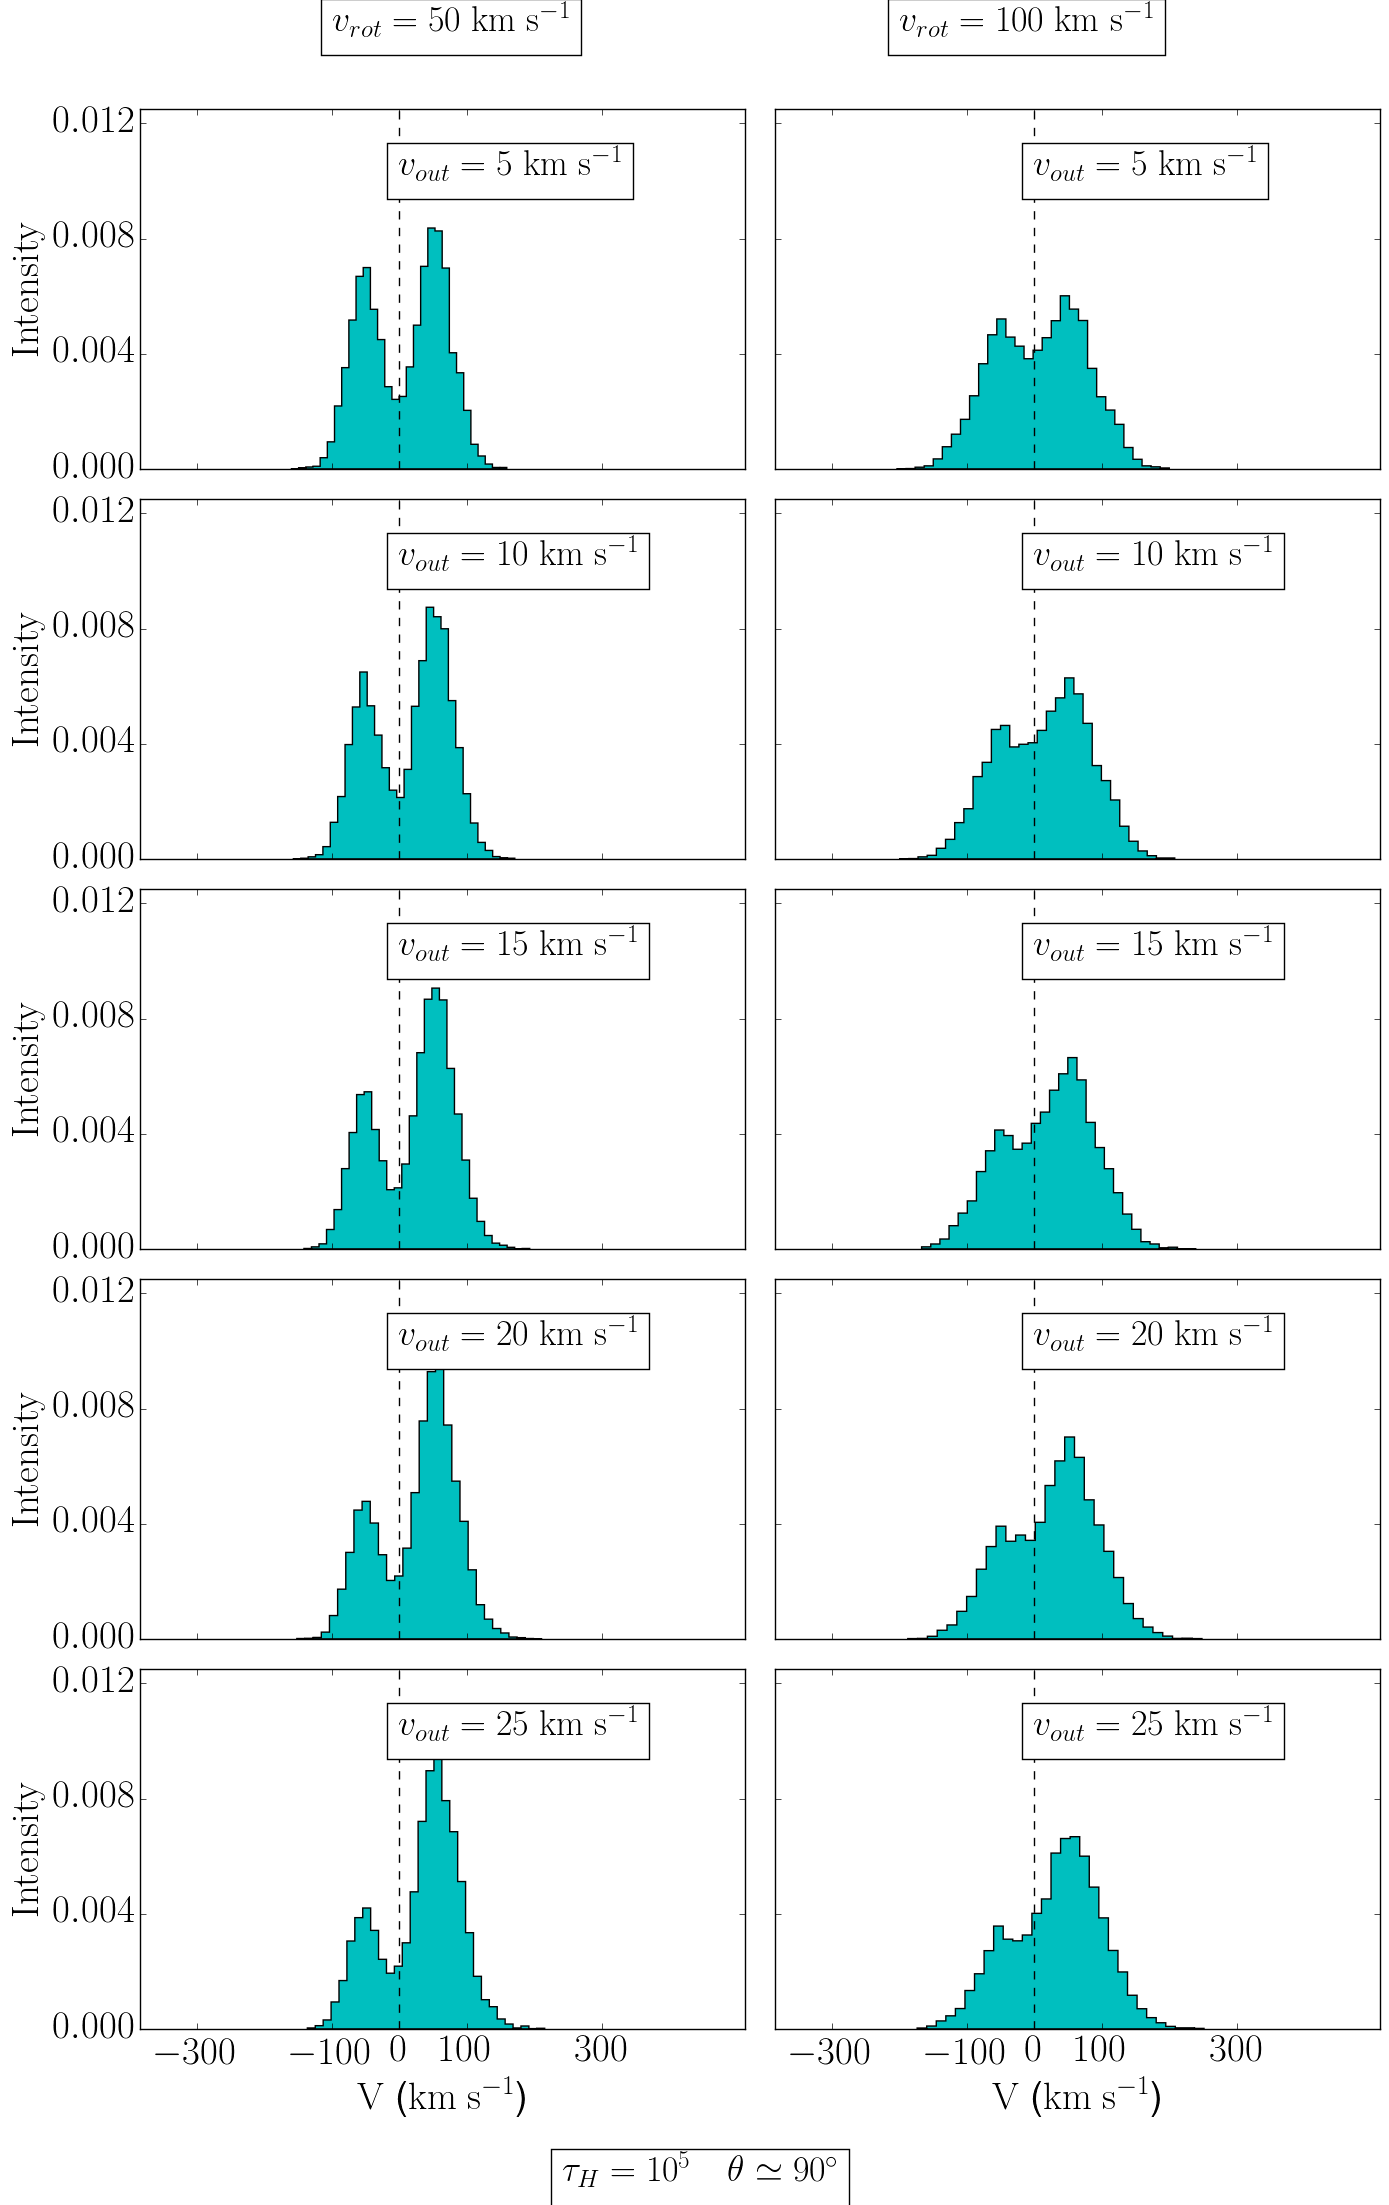
\includegraphics[width=0.95\textwidth]{./figures/chapter3/3_tau10E5_phi83-90}
	\end{center}
	\caption{\textbf{\lya profile for \tauh$=10^5$:} With \vrot ranging $50,100$ \kms and \vout ranging $5,10,15,20,25$ \kms. The intensity is in arbitrary units.
		\label{fig:3_tau10E5_phi83-90}}
\end{figure}

\newpage

\begin{figure}[h!]
	\begin{center}
		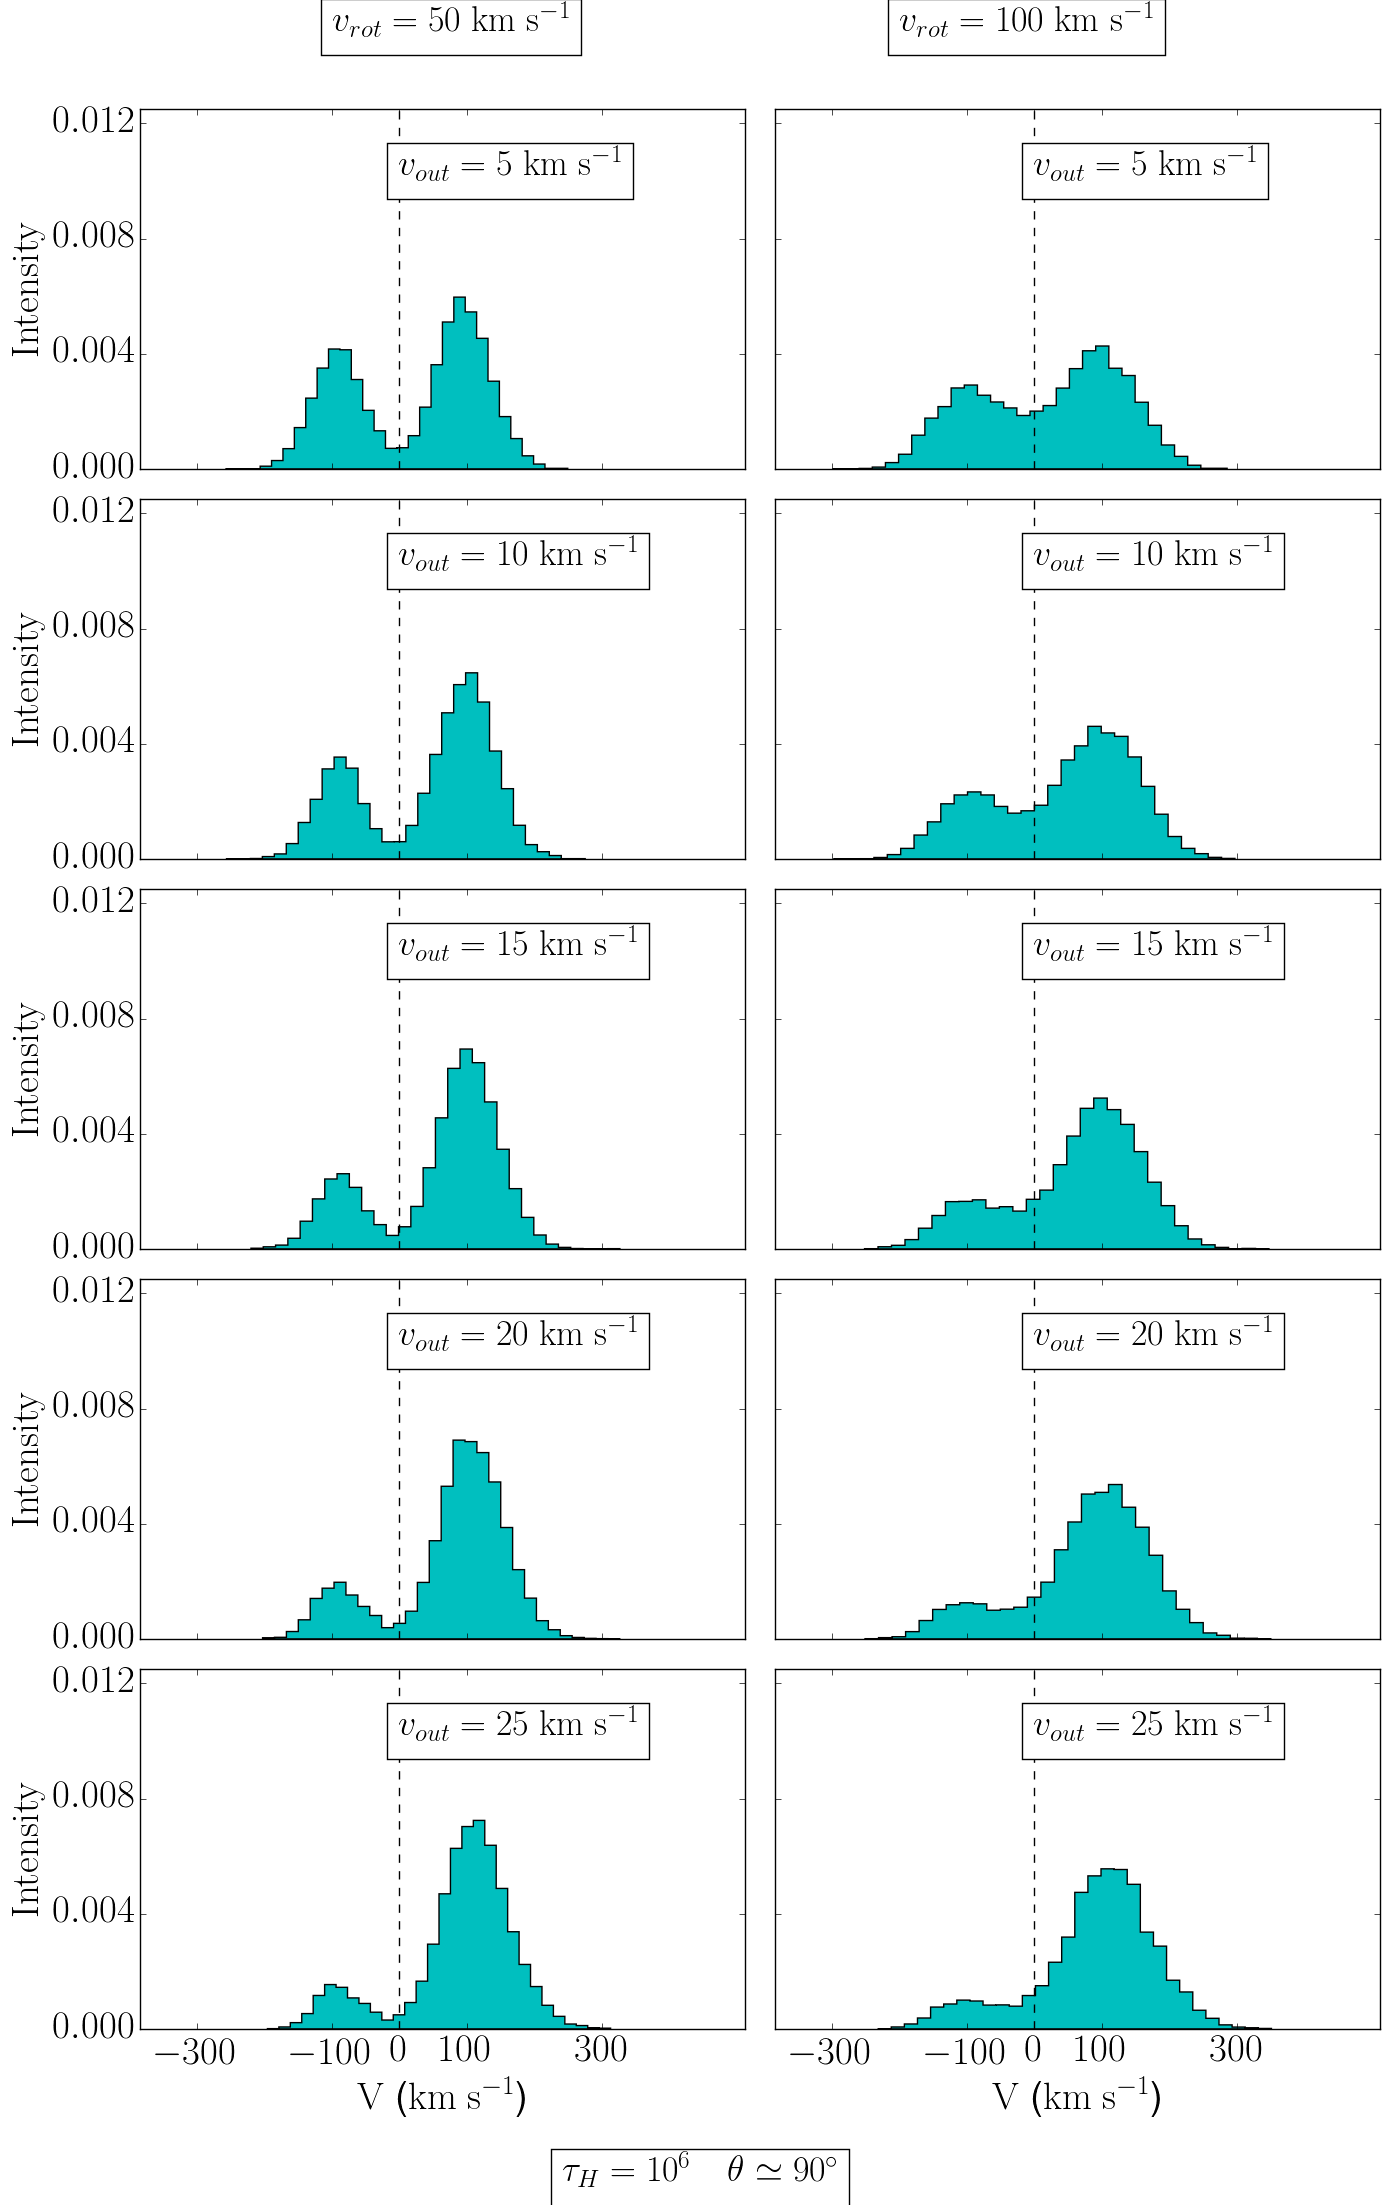
\includegraphics[width=0.95\textwidth]{./figures/chapter3/3_tau10E6_phi83-90}
	\end{center}
	\caption{\textbf{\lya profile for \tauh$=10^6$:} With \vrot ranging $50,100$ \kms and \vout ranging $5,10,15,20,25$ \kms. The intensity is in arbitrary units.
		\label{fig:3_tau10E6_phi83-90}}
\end{figure}

\newpage

\begin{figure}[h!]
	\begin{center}
		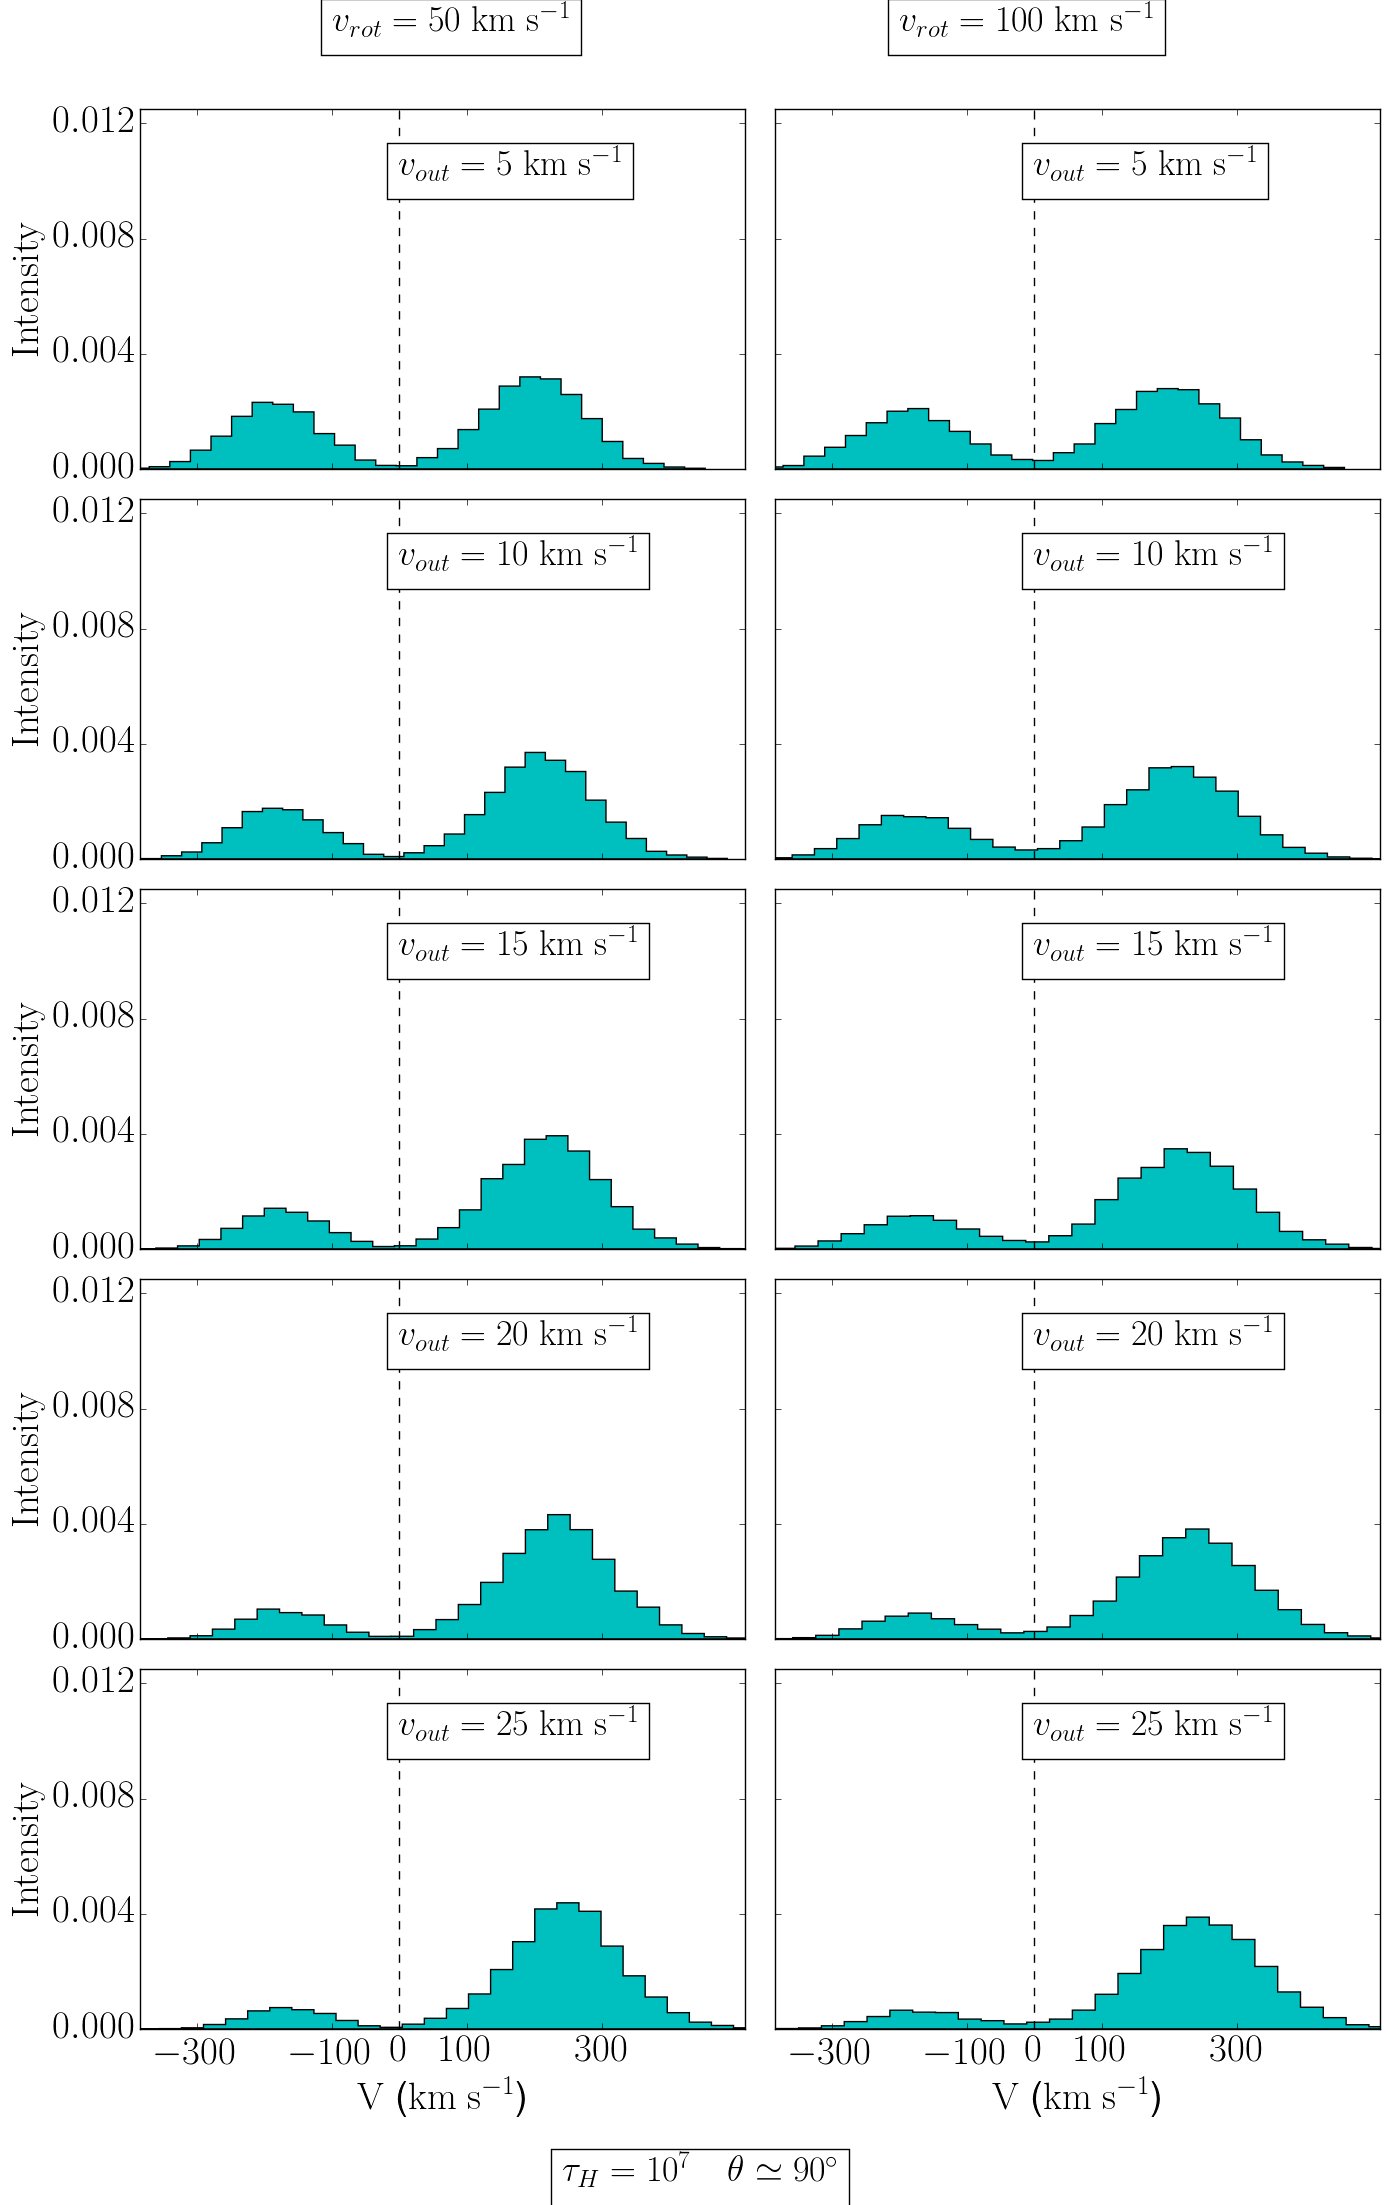
\includegraphics[width=0.95\textwidth]{./figures/chapter3/3_tau10E7_phi83-90}
	\end{center}
	\caption{\textbf{\lya profile for \tauh$=10^7$:} With \vrot ranging $50,100$ \kms and \vout ranging $5,10,15,20,25$ \kms. The intensity is in arbitrary units.
		\label{fig:3_tau10E7_phi83-90}}
\end{figure}

\newpage

From the figures I can confirm that only a little fraction of \vrot, in the radial direction, is necessary to obtain 2 asymmetric peaks. This final spectra are very consistent with LAEs renowned observations.  \\


\section{Influence of the viewing angle $\theta$}
As stated in the preceding chapter, I have to take into account the viewing angle of the galaxy to create the resulting spectra. For all of the parameters' combinations, the effect of $\theta$ in the \lya line is always the same.\\

\begin{figure}[h!]
	\begin{center}
		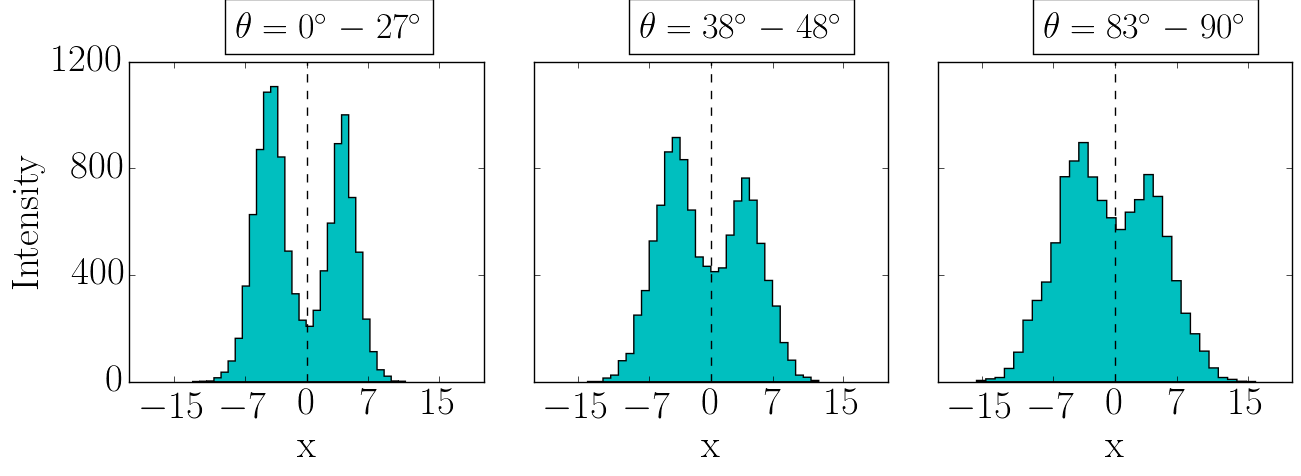
\includegraphics[width=1\textwidth]{./figures/chapter3/influence_viewing_angle2}
	\end{center}
	\caption{\textbf{\lya profile for different $\theta$:} With \tauh$=10^5$, \vrot$=50$ \kms and \vout$=20$ \kms.The intensity is in arbitrary units.
		\label{fig:influence_viewing_angle}}
\end{figure}

In order to exemplify, I use the particular case of \tauh$=10^5$, \vrot$=50$ \kms and \vout$=20$ \kms. As seen in Fig. \ref{fig:influence_viewing_angle} it is very clear that the intensity of the valley between the two peaks is increased along with $\theta$. This causes an intensity decrease in the rest of the frequencies, thus a broadening of the line. \\

It is important to note that I show only the results of a particular range of $\theta$. I choose the range in which I see the galaxy's angular momentum vector going perpendicular to my relative position vector (i.e. $\theta \in [83^\circ,96^\circ]$). This choice is with the purpose of decreasing the number of plots in the document. However, I ensure the reader there is an analogous behavior for all of the ranges. \\

\section{Morphology of \lya line}
After obtaining logical and observation-consistent results in the \lya line, it is necessary to quantify its morphology. This is done with 3 different factors: the standard deviation ($\mathrm{std}$), the skewness ($\mathrm{skw}$) and a factor sigma of asymmetry ($\sigma_A$). \\

\subsection{Standard Deviation}
In this part I use the $\mathrm{std}$ to estimate the dispersion of the frequencies in the \lya line. It is important to recall that if the value is close to zero, then the frequencies tend to be very close to their expected value. If it increases, it means the frequencies are spreading to wider ranges. \\

\begin{figure}[h!]
	\begin{center}
		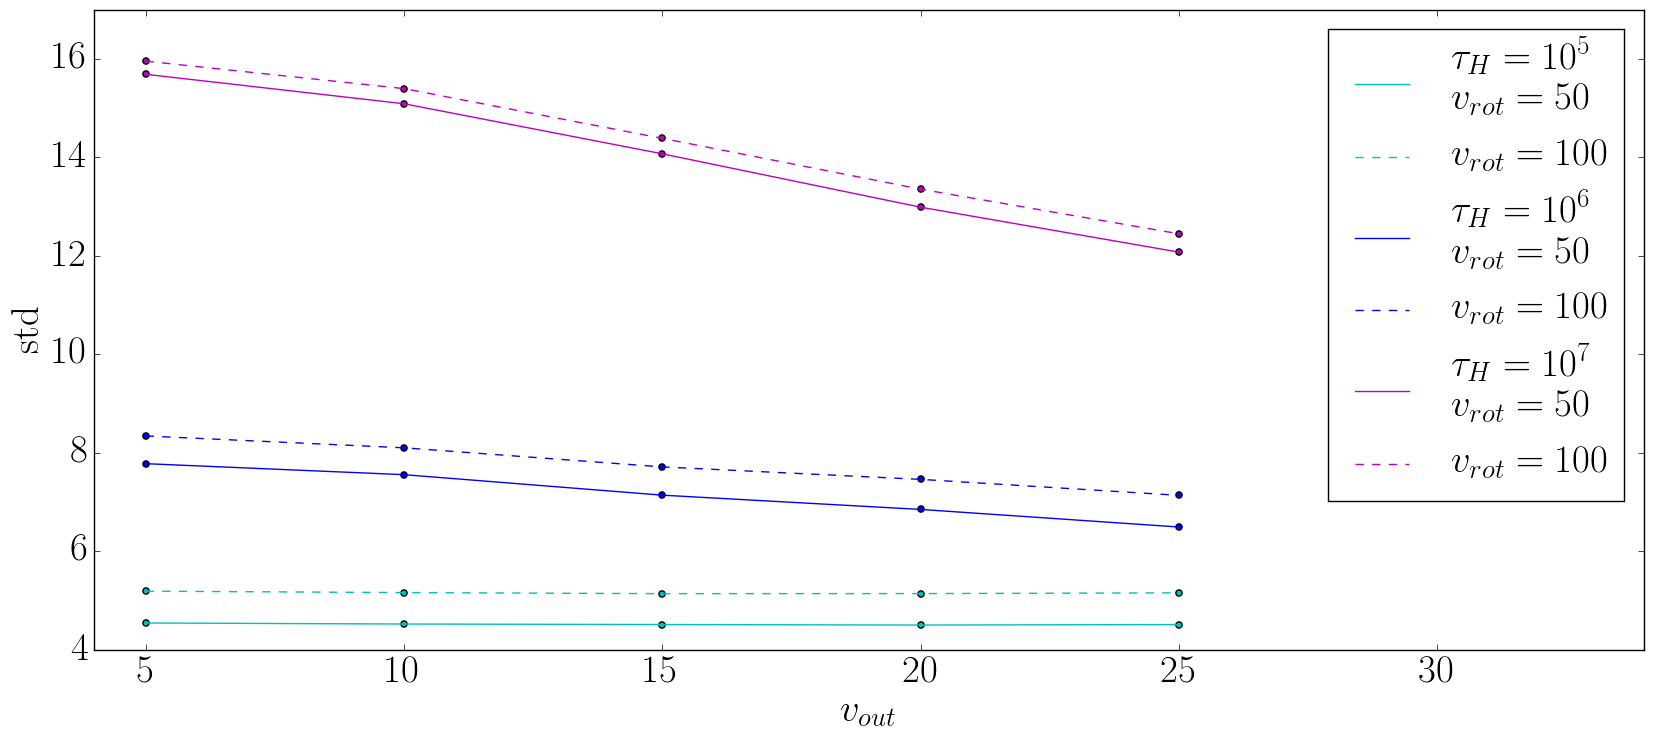
\includegraphics[width=1\textwidth]{./figures/chapter3/std}
	\end{center}
	\caption{\textbf{Standard deviation plot for each \tauh. The units of \vrot and \vout are \kms}
	\label{fig:std}}
\end{figure}

As seen in Fig. \ref{fig:std}, the standard deviation is inversely proportional to the outflow velocity. Also, the higher the \tauh, the more inclined the curves. This implies that the greater \vout is, the less disperse is the \lya frequency distribution. This clearly shows that the peaks start merging to one another if \vout is increasing.\\

\subsection{Skewness}
In this part I use the $\mathrm{skw}$ to estimate the asymmetry of the \lya line. Is important to recall that if the value is greater than zero, there is more weight in the left tail of the line. And on the contrary, if it is less than zero, there is more weight in the right one.\\

\begin{figure}[h!]
	\begin{center}
		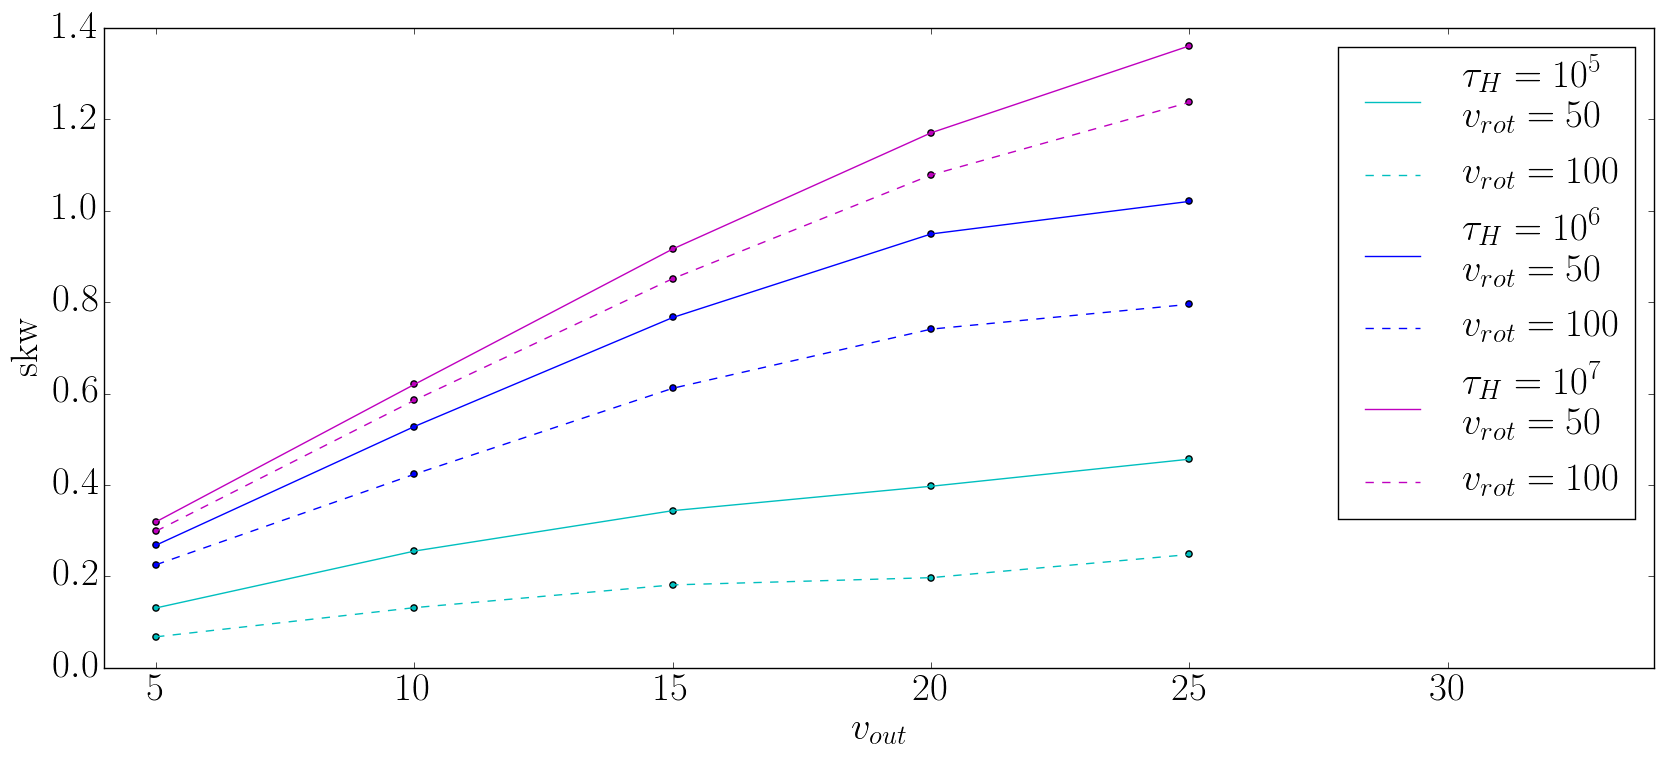
\includegraphics[width=1\textwidth]{./figures/chapter3/skw}
	\end{center}
	\caption{\textbf{Skewness plot for each \tauh. The units of \vrot and \vout are \kms} 
		\label{fig:skw}}
\end{figure}

As seen in Fig. \ref{fig:skw}, the skewness is proportional to the outflow velocity. This implies that the greater \vout is, the more asymmetric is the \lya frequency distribution.\\

\subsection{Sigma of Asymmetry}
In this part I use the $\sigma_A$ factor to estimate in another way the asymmetry of the \lya line. This was defined by (MISSING REFERENCE) as follows. The two peaks, the left one and the right one, are fitted with a Gaussian curve. Their standard deviations $\sigma_{left}$ and $\sigma_{right}$ are obtained. Then the factor $\sigma_A$ is:

\begin{equation}
\sigma_A = \frac{\sigma_{right}}{\sigma_{left}}
\end{equation}

Is important to recall that if the value is greater than one, the left peak is thiner than the right peak. And if it is less than one, there left peak is wider than the right peak.\\

(MISSING PLOTS)
%https://github.com/mariacamilaremolinagutierrez/RotationOutflowLymanAlpha/blob/master/Simulation/PeaksAsymmetry.ipynb

\section{Influences of the free parameters}

\subsection{Influence of the Galaxy Optical Depth: \tauh}
The influence of \tauh in the \lya line can be seen clearly in figures (Fig. \ref{fig:1_tau10E5_phi83-90} \ref{fig:1_tau10E6_phi83-90} \ref{fig:1_tau10E7_phi83-90}). What the optical depth causes is that the more \tauh there is, the more redshifted is the line respect to the zero value of $x$. This result has been previously obtained. So, my results are consistent with literature regarding this parameter.\\

\subsection{Influence of the Galaxy Outflow Velocity: \vout}
The influence of \vout is very clear since the first run. When this outflows velocity increases, the right peak of the spectrum goes down in intensity until it merges with the left peak.  This result has also been previously obtained. So, my results are consistent with literature regarding this other parameter.\\

\subsection{Influence of the Galaxy Rotation Velocity: \vrot}
The influence of \vrot is slightly clear because of the giant impact \vout has. However it is noticeable that the \lya line broadens and lowers intensity when the rotation velocity increases. This effect has been less studied in literature. Only Garavito et al. \cite{Garavito14} has simulated its effect, but our results are consistent. 